\PassOptionsToPackage{dvipsnames,table}{xcolor}
\documentclass[10pt]{beamer}
\usepackage{Cours}

\begin{document}


\newcounter{numchap}
\setcounter{numchap}{1}
\newcounter{numframe}
\setcounter{numframe}{0}
\newcommand{\mframe}[1]{\frametitle{#1} \addtocounter{numframe}{1}}
\newcommand{\cnum}{\fbox{\textcolor{yellow}{\textbf{C\thenumchap}}}~}
\newcommand{\makess}[1]{\section{#1} \label{ss\thesection}}
\newcommand{\stitle}{\textcolor{yellow}{\textbf{\thesection. \nameref{ss\thesection}}}}

\definecolor{codebg}{gray}{0.90}
\definecolor{grispale}{gray}{0.95}
\definecolor{fluo}{rgb}{1,0.96,0.62}
\newminted[langageC]{c}{linenos=true,escapeinside=||,highlightcolor=fluo,tabsize=2,breaklines=true}
\newminted[codepython]{python}{linenos=true,escapeinside=||,highlightcolor=fluo,tabsize=2,breaklines=true}
% Inclusion complète (ou partiel en indiquant premiere et dernière ligne) d'un fichier C
\newcommand{\inputC}[3]{\begin{mdframed}[backgroundcolor=codebg] \inputminted[breaklines=true,fontsize=#3,linenos=true,highlightcolor=fluo,tabsize=2,highlightlines={#2}]{c}{#1} \end{mdframed}}
\newcommand{\inputpartC}[5]{\begin{mdframed}[backgroundcolor=codebg] \inputminted[breaklines=true,fontsize=#3,linenos=true,highlightcolor=fluo,tabsize=2,highlightlines={#2},firstline=#4,lastline=#5,firstnumber=1]{c}{#1} \end{mdframed}}
\newcommand{\inputpython}[3]{\begin{mdframed}[backgroundcolor=codebg] \inputminted[breaklines=true,fontsize=#3,linenos=true,highlightcolor=fluo,tabsize=2,highlightlines={#2}]{python}{#1} \end{mdframed}}
\newcommand{\inputpartOCaml}[5]{\begin{mdframed}[backgroundcolor=codebg] \inputminted[breaklines=true,fontsize=#3,linenos=true,highlightcolor=fluo,tabsize=2,highlightlines={#2},firstline=#4,lastline=#5,firstnumber=1]{OCaml}{#1} \end{mdframed}}
\BeforeBeginEnvironment{minted}{\begin{mdframed}[backgroundcolor=codebg]}
\AfterEndEnvironment{minted}{\end{mdframed}}
\newcommand{\kw}[1]{\textcolor{blue}{\tt #1}}

\newtcolorbox{rcadre}[4]{halign=center,colback={#1},colframe={#2},width={#3cm},height={#4cm},valign=center,boxrule=1pt,left=0pt,right=0pt}
\newtcolorbox{cadre}[4]{halign=center,colback={#1},colframe={#2},arc=0mm,width={#3cm},height={#4cm},valign=center,boxrule=1pt,left=0pt,right=0pt}
\newcommand{\myem}[1]{\colorbox{fluo}{#1}}
\mdfsetup{skipabove=1pt,skipbelow=-2pt}



% Noeud dans un cadre pour les arbres
\newcommand{\noeud}[2]{\Tr{\fbox{\textcolor{#1}{\tt #2}}}}

\newcommand{\htmlmode}{\lstset{language=html,numbers=left, tabsize=4, frame=single, breaklines=true, keywordstyle=\ttfamily, basicstyle=\small,
   numberstyle=\tiny\ttfamily, framexleftmargin=0mm, backgroundcolor=\color{grispale}, xleftmargin=12mm,showstringspaces=false}}
\newcommand{\pythonmode}{\lstset{
   language=python,
   linewidth=\linewidth,
   numbers=left,
   tabsize=4,
   frame=single,
   breaklines=true,
   keywordstyle=\ttfamily\color{blue},
   basicstyle=\small,
   numberstyle=\tiny\ttfamily,
   framexleftmargin=-2mm,
   numbersep=-0.5mm,
   backgroundcolor=\color{codebg},
   xleftmargin=-1mm, 
   showstringspaces=false,
   commentstyle=\color{gray},
   stringstyle=\color{OliveGreen},
   emph={turtle,Screen,Turtle},
   emphstyle=\color{RawSienna},
   morekeywords={setheading,goto,backward,forward,left,right,pendown,penup,pensize,color,speed,hideturtle,showturtle,forward}}
   }
   \newcommand{\Cmode}{\lstset{
      language=[ANSI]C,
      linewidth=\linewidth,
      numbers=left,
      tabsize=4,
      frame=single,
      breaklines=true,
      keywordstyle=\ttfamily\color{blue},
      basicstyle=\small,
      numberstyle=\tiny\ttfamily,
      framexleftmargin=0mm,
      numbersep=2mm,
      backgroundcolor=\color{codebg},
      xleftmargin=0mm, 
      showstringspaces=false,
      commentstyle=\color{gray},
      stringstyle=\color{OliveGreen},
      emphstyle=\color{RawSienna},
      escapechar=\|,
      morekeywords={}}
      }
\newcommand{\bashmode}{\lstset{language=bash,numbers=left, tabsize=2, frame=single, breaklines=true, basicstyle=\ttfamily,
   numberstyle=\tiny\ttfamily, framexleftmargin=0mm, backgroundcolor=\color{grispale}, xleftmargin=12mm, showstringspaces=false}}
\newcommand{\exomode}{\lstset{language=python,numbers=left, tabsize=2, frame=single, breaklines=true, basicstyle=\ttfamily,
   numberstyle=\tiny\ttfamily, framexleftmargin=13mm, xleftmargin=12mm, basicstyle=\small, showstringspaces=false}}
   
   
  
%tei pour placer les images
%tei{nom de l’image}{échelle de l’image}{sens}{texte a positionner}
%sens ="1" (droite) ou "2" (gauche)
\newlength{\ltxt}
\newcommand{\tei}[4]{
\setlength{\ltxt}{\linewidth}
\setbox0=\hbox{\includegraphics[scale=#2]{#1}}
\addtolength{\ltxt}{-\wd0}
\addtolength{\ltxt}{-10pt}
\ifthenelse{\equal{#3}{1}}{
\begin{minipage}{\wd0}
\includegraphics[scale=#2]{#1}
\end{minipage}
\hfill
\begin{minipage}{\ltxt}
#4
\end{minipage}
}{
\begin{minipage}{\ltxt}
#4
\end{minipage}
\hfill
\begin{minipage}{\wd0}
\includegraphics[scale=#2]{#1}
\end{minipage}
}
}

%Juxtaposition d'une image pspciture et de texte 
%#1: = code pstricks de l'image
%#2: largeur de l'image
%#3: hauteur de l'image
%#4: Texte à écrire
\newcommand{\ptp}[4]{
\setlength{\ltxt}{\linewidth}
\addtolength{\ltxt}{-#2 cm}
\addtolength{\ltxt}{-0.1 cm}
\begin{minipage}[b][#3 cm][t]{\ltxt}
#4
\end{minipage}\hfill
\begin{minipage}[b][#3 cm][c]{#2 cm}
#1
\end{minipage}\par
}



%Macros pour les graphiques
\psset{linewidth=0.5\pslinewidth,PointSymbol=x}
\setlength{\fboxrule}{0.5pt}
\newcounter{tempangle}

%Marque la longueur du segment d'extrémité  #1 et  #2 avec la valeur #3, #4 est la distance par rapport au segment (en %age de la valeur de celui ci) et #5 l'orientation du marquage : +90 ou -90
\newcommand{\afflong}[5]{
\pstRotation[RotAngle=#4,PointSymbol=none,PointName=none]{#1}{#2}[X] 
\pstHomO[PointSymbol=none,PointName=none,HomCoef=#5]{#1}{X}[Y]
\pstTranslation[PointSymbol=none,PointName=none]{#1}{#2}{Y}[Z]
 \ncline{|<->|,linewidth=0.25\pslinewidth}{Y}{Z} \ncput*[nrot=:U]{\footnotesize{#3}}
}
\newcommand{\afflongb}[3]{
\ncline{|<->|,linewidth=0}{#1}{#2} \naput*[nrot=:U]{\footnotesize{#3}}
}

%Construis le point #4 situé à #2 cm du point #1 avant un angle #3 par rapport à l'horizontale. #5 = liste de paramètre
\newcommand{\lsegment}[5]{\pstGeonode[PointSymbol=none,PointName=none](0,0){O'}(#2,0){I'} \pstTranslation[PointSymbol=none,PointName=none]{O'}{I'}{#1}[J'] \pstRotation[RotAngle=#3,PointSymbol=x,#5]{#1}{J'}[#4]}
\newcommand{\tsegment}[5]{\pstGeonode[PointSymbol=none,PointName=none](0,0){O'}(#2,0){I'} \pstTranslation[PointSymbol=none,PointName=none]{O'}{I'}{#1}[J'] \pstRotation[RotAngle=#3,PointSymbol=x,#5]{#1}{J'}[#4] \pstLineAB{#4}{#1}}

%Construis le point #4 situé à #3 cm du point #1 et faisant un angle de  90° avec la droite (#1,#2) #5 = liste de paramètre
\newcommand{\psegment}[5]{
\pstGeonode[PointSymbol=none,PointName=none](0,0){O'}(#3,0){I'}
 \pstTranslation[PointSymbol=none,PointName=none]{O'}{I'}{#1}[J']
 \pstInterLC[PointSymbol=none,PointName=none]{#1}{#2}{#1}{J'}{M1}{M2} \pstRotation[RotAngle=-90,PointSymbol=x,#5]{#1}{M1}[#4]
  }
  
%Construis le point #4 situé à #3 cm du point #1 et faisant un angle de  #5° avec la droite (#1,#2) #6 = liste de paramètre
\newcommand{\mlogo}[6]{
\pstGeonode[PointSymbol=none,PointName=none](0,0){O'}(#3,0){I'}
 \pstTranslation[PointSymbol=none,PointName=none]{O'}{I'}{#1}[J']
 \pstInterLC[PointSymbol=none,PointName=none]{#1}{#2}{#1}{J'}{M1}{M2} \pstRotation[RotAngle=#5,PointSymbol=x,#6]{#1}{M2}[#4]
  }

% Construis un triangle avec #1=liste des 3 sommets séparés par des virgules, #2=liste des 3 longueurs séparés par des virgules, #3 et #4 : paramètre d'affichage des 2e et 3 points et #5 : inclinaison par rapport à l'horizontale
%autre macro identique mais sans tracer les segments joignant les sommets
\noexpandarg
\newcommand{\Triangleccc}[5]{
\StrBefore{#1}{,}[\pointA]
\StrBetween[1,2]{#1}{,}{,}[\pointB]
\StrBehind[2]{#1}{,}[\pointC]
\StrBefore{#2}{,}[\coteA]
\StrBetween[1,2]{#2}{,}{,}[\coteB]
\StrBehind[2]{#2}{,}[\coteC]
\tsegment{\pointA}{\coteA}{#5}{\pointB}{#3} 
\lsegment{\pointA}{\coteB}{0}{Z1}{PointSymbol=none, PointName=none}
\lsegment{\pointB}{\coteC}{0}{Z2}{PointSymbol=none, PointName=none}
\pstInterCC{\pointA}{Z1}{\pointB}{Z2}{\pointC}{Z3} 
\pstLineAB{\pointA}{\pointC} \pstLineAB{\pointB}{\pointC}
\pstSymO[PointName=\pointC,#4]{C}{C}[C]
}
\noexpandarg
\newcommand{\TrianglecccP}[5]{
\StrBefore{#1}{,}[\pointA]
\StrBetween[1,2]{#1}{,}{,}[\pointB]
\StrBehind[2]{#1}{,}[\pointC]
\StrBefore{#2}{,}[\coteA]
\StrBetween[1,2]{#2}{,}{,}[\coteB]
\StrBehind[2]{#2}{,}[\coteC]
\tsegment{\pointA}{\coteA}{#5}{\pointB}{#3} 
\lsegment{\pointA}{\coteB}{0}{Z1}{PointSymbol=none, PointName=none}
\lsegment{\pointB}{\coteC}{0}{Z2}{PointSymbol=none, PointName=none}
\pstInterCC[PointNameB=none,PointSymbolB=none,#4]{\pointA}{Z1}{\pointB}{Z2}{\pointC}{Z1} 
}


% Construis un triangle avec #1=liste des 3 sommets séparés par des virgules, #2=liste formée de 2 longueurs et d'un angle séparés par des virgules, #3 et #4 : paramètre d'affichage des 2e et 3 points et #5 : inclinaison par rapport à l'horizontale
%autre macro identique mais sans tracer les segments joignant les sommets
\newcommand{\Trianglecca}[5]{
\StrBefore{#1}{,}[\pointA]
\StrBetween[1,2]{#1}{,}{,}[\pointB]
\StrBehind[2]{#1}{,}[\pointC]
\StrBefore{#2}{,}[\coteA]
\StrBetween[1,2]{#2}{,}{,}[\coteB]
\StrBehind[2]{#2}{,}[\angleA]
\tsegment{\pointA}{\coteA}{#5}{\pointB}{#3} 
\setcounter{tempangle}{#5}
\addtocounter{tempangle}{\angleA}
\tsegment{\pointA}{\coteB}{\thetempangle}{\pointC}{#4}
\pstLineAB{\pointB}{\pointC}
}
\newcommand{\TriangleccaP}[5]{
\StrBefore{#1}{,}[\pointA]
\StrBetween[1,2]{#1}{,}{,}[\pointB]
\StrBehind[2]{#1}{,}[\pointC]
\StrBefore{#2}{,}[\coteA]
\StrBetween[1,2]{#2}{,}{,}[\coteB]
\StrBehind[2]{#2}{,}[\angleA]
\lsegment{\pointA}{\coteA}{#5}{\pointB}{#3} 
\setcounter{tempangle}{#5}
\addtocounter{tempangle}{\angleA}
\lsegment{\pointA}{\coteB}{\thetempangle}{\pointC}{#4}
}

% Construis un triangle avec #1=liste des 3 sommets séparés par des virgules, #2=liste formée de 1 longueurs et de deux angle séparés par des virgules, #3 et #4 : paramètre d'affichage des 2e et 3 points et #5 : inclinaison par rapport à l'horizontale
%autre macro identique mais sans tracer les segments joignant les sommets
\newcommand{\Trianglecaa}[5]{
\StrBefore{#1}{,}[\pointA]
\StrBetween[1,2]{#1}{,}{,}[\pointB]
\StrBehind[2]{#1}{,}[\pointC]
\StrBefore{#2}{,}[\coteA]
\StrBetween[1,2]{#2}{,}{,}[\angleA]
\StrBehind[2]{#2}{,}[\angleB]
\tsegment{\pointA}{\coteA}{#5}{\pointB}{#3} 
\setcounter{tempangle}{#5}
\addtocounter{tempangle}{\angleA}
\lsegment{\pointA}{1}{\thetempangle}{Z1}{PointSymbol=none, PointName=none}
\setcounter{tempangle}{#5}
\addtocounter{tempangle}{180}
\addtocounter{tempangle}{-\angleB}
\lsegment{\pointB}{1}{\thetempangle}{Z2}{PointSymbol=none, PointName=none}
\pstInterLL[#4]{\pointA}{Z1}{\pointB}{Z2}{\pointC}
\pstLineAB{\pointA}{\pointC}
\pstLineAB{\pointB}{\pointC}
}
\newcommand{\TrianglecaaP}[5]{
\StrBefore{#1}{,}[\pointA]
\StrBetween[1,2]{#1}{,}{,}[\pointB]
\StrBehind[2]{#1}{,}[\pointC]
\StrBefore{#2}{,}[\coteA]
\StrBetween[1,2]{#2}{,}{,}[\angleA]
\StrBehind[2]{#2}{,}[\angleB]
\lsegment{\pointA}{\coteA}{#5}{\pointB}{#3} 
\setcounter{tempangle}{#5}
\addtocounter{tempangle}{\angleA}
\lsegment{\pointA}{1}{\thetempangle}{Z1}{PointSymbol=none, PointName=none}
\setcounter{tempangle}{#5}
\addtocounter{tempangle}{180}
\addtocounter{tempangle}{-\angleB}
\lsegment{\pointB}{1}{\thetempangle}{Z2}{PointSymbol=none, PointName=none}
\pstInterLL[#4]{\pointA}{Z1}{\pointB}{Z2}{\pointC}
}

%Construction d'un cercle de centre #1 et de rayon #2 (en cm)
\newcommand{\Cercle}[2]{
\lsegment{#1}{#2}{0}{Z1}{PointSymbol=none, PointName=none}
\pstCircleOA{#1}{Z1}
}

%construction d'un parallélogramme #1 = liste des sommets, #2 = liste contenant les longueurs de 2 côtés consécutifs et leurs angles;  #3, #4 et #5 : paramètre d'affichage des sommets #6 inclinaison par rapport à l'horizontale 
% meme macro sans le tracé des segements
\newcommand{\Para}[6]{
\StrBefore{#1}{,}[\pointA]
\StrBetween[1,2]{#1}{,}{,}[\pointB]
\StrBetween[2,3]{#1}{,}{,}[\pointC]
\StrBehind[3]{#1}{,}[\pointD]
\StrBefore{#2}{,}[\longueur]
\StrBetween[1,2]{#2}{,}{,}[\largeur]
\StrBehind[2]{#2}{,}[\angle]
\tsegment{\pointA}{\longueur}{#6}{\pointB}{#3} 
\setcounter{tempangle}{#6}
\addtocounter{tempangle}{\angle}
\tsegment{\pointA}{\largeur}{\thetempangle}{\pointD}{#5}
\pstMiddleAB[PointName=none,PointSymbol=none]{\pointB}{\pointD}{Z1}
\pstSymO[#4]{Z1}{\pointA}[\pointC]
\pstLineAB{\pointB}{\pointC}
\pstLineAB{\pointC}{\pointD}
}
\newcommand{\ParaP}[6]{
\StrBefore{#1}{,}[\pointA]
\StrBetween[1,2]{#1}{,}{,}[\pointB]
\StrBetween[2,3]{#1}{,}{,}[\pointC]
\StrBehind[3]{#1}{,}[\pointD]
\StrBefore{#2}{,}[\longueur]
\StrBetween[1,2]{#2}{,}{,}[\largeur]
\StrBehind[2]{#2}{,}[\angle]
\lsegment{\pointA}{\longueur}{#6}{\pointB}{#3} 
\setcounter{tempangle}{#6}
\addtocounter{tempangle}{\angle}
\lsegment{\pointA}{\largeur}{\thetempangle}{\pointD}{#5}
\pstMiddleAB[PointName=none,PointSymbol=none]{\pointB}{\pointD}{Z1}
\pstSymO[#4]{Z1}{\pointA}[\pointC]
}


%construction d'un cerf-volant #1 = liste des sommets, #2 = liste contenant les longueurs de 2 côtés consécutifs et leurs angles;  #3, #4 et #5 : paramètre d'affichage des sommets #6 inclinaison par rapport à l'horizontale 
% meme macro sans le tracé des segements
\newcommand{\CerfVolant}[6]{
\StrBefore{#1}{,}[\pointA]
\StrBetween[1,2]{#1}{,}{,}[\pointB]
\StrBetween[2,3]{#1}{,}{,}[\pointC]
\StrBehind[3]{#1}{,}[\pointD]
\StrBefore{#2}{,}[\longueur]
\StrBetween[1,2]{#2}{,}{,}[\largeur]
\StrBehind[2]{#2}{,}[\angle]
\tsegment{\pointA}{\longueur}{#6}{\pointB}{#3} 
\setcounter{tempangle}{#6}
\addtocounter{tempangle}{\angle}
\tsegment{\pointA}{\largeur}{\thetempangle}{\pointD}{#5}
\pstOrtSym[#4]{\pointB}{\pointD}{\pointA}[\pointC]
\pstLineAB{\pointB}{\pointC}
\pstLineAB{\pointC}{\pointD}
}

%construction d'un quadrilatère quelconque #1 = liste des sommets, #2 = liste contenant les longueurs des 4 côtés et l'angle entre 2 cotés consécutifs  #3, #4 et #5 : paramètre d'affichage des sommets #6 inclinaison par rapport à l'horizontale 
% meme macro sans le tracé des segements
\newcommand{\Quadri}[6]{
\StrBefore{#1}{,}[\pointA]
\StrBetween[1,2]{#1}{,}{,}[\pointB]
\StrBetween[2,3]{#1}{,}{,}[\pointC]
\StrBehind[3]{#1}{,}[\pointD]
\StrBefore{#2}{,}[\coteA]
\StrBetween[1,2]{#2}{,}{,}[\coteB]
\StrBetween[2,3]{#2}{,}{,}[\coteC]
\StrBetween[3,4]{#2}{,}{,}[\coteD]
\StrBehind[4]{#2}{,}[\angle]
\tsegment{\pointA}{\coteA}{#6}{\pointB}{#3} 
\setcounter{tempangle}{#6}
\addtocounter{tempangle}{\angle}
\tsegment{\pointA}{\coteD}{\thetempangle}{\pointD}{#5}
\lsegment{\pointB}{\coteB}{0}{Z1}{PointSymbol=none, PointName=none}
\lsegment{\pointD}{\coteC}{0}{Z2}{PointSymbol=none, PointName=none}
\pstInterCC[PointNameA=none,PointSymbolA=none,#4]{\pointB}{Z1}{\pointD}{Z2}{Z3}{\pointC} 
\pstLineAB{\pointB}{\pointC}
\pstLineAB{\pointC}{\pointD}
}


% Définition des colonnes centrées ou à droite pour tabularx
\newcolumntype{Y}{>{\centering\arraybackslash}X}
\newcolumntype{Z}{>{\flushright\arraybackslash}X}

%Les pointillés à remplir par les élèves
\newcommand{\po}[1]{\makebox[#1 cm]{\dotfill}}
\newcommand{\lpo}[1][3]{%
\multido{}{#1}{\makebox[\linewidth]{\dotfill}
}}

%Liste des pictogrammes utilisés sur la fiche d'exercice ou d'activités
\newcommand{\bombe}{\faBomb}
\newcommand{\livre}{\faBook}
\newcommand{\calculatrice}{\faCalculator}
\newcommand{\oral}{\faCommentO}
\newcommand{\surfeuille}{\faEdit}
\newcommand{\ordinateur}{\faLaptop}
\newcommand{\ordi}{\faDesktop}
\newcommand{\ciseaux}{\faScissors}
\newcommand{\danger}{\faExclamationTriangle}
\newcommand{\out}{\faSignOut}
\newcommand{\cadeau}{\faGift}
\newcommand{\flash}{\faBolt}
\newcommand{\lumiere}{\faLightbulb}
\newcommand{\compas}{\dsmathematical}
\newcommand{\calcullitteral}{\faTimesCircleO}
\newcommand{\raisonnement}{\faCogs}
\newcommand{\recherche}{\faSearch}
\newcommand{\rappel}{\faHistory}
\newcommand{\video}{\faFilm}
\newcommand{\capacite}{\faPuzzlePiece}
\newcommand{\aide}{\faLifeRing}
\newcommand{\loin}{\faExternalLink}
\newcommand{\groupe}{\faUsers}
\newcommand{\bac}{\faGraduationCap}
\newcommand{\histoire}{\faUniversity}
\newcommand{\coeur}{\faSave}
\newcommand{\python}{\faPython}
\newcommand{\os}{\faMicrochip}
\newcommand{\rd}{\faCubes}
\newcommand{\data}{\faColumns}
\newcommand{\web}{\faCode}
\newcommand{\prog}{\faFile}
\newcommand{\algo}{\faCogs}
\newcommand{\important}{\faExclamationCircle}
\newcommand{\maths}{\faTimesCircle}
% Traitement des données en tables
\newcommand{\tables}{\faColumns}
% Types construits
\newcommand{\construits}{\faCubes}
% Type et valeurs de base
\newcommand{\debase}{{\footnotesize \faCube}}
% Systèmes d'exploitation
\newcommand{\linux}{\faLinux}
\newcommand{\sd}{\faProjectDiagram}
\newcommand{\bd}{\faDatabase}

%Les ensembles de nombres
\renewcommand{\N}{\mathbb{N}}
\newcommand{\D}{\mathbb{D}}
\newcommand{\Z}{\mathbb{Z}}
\newcommand{\Q}{\mathbb{Q}}
\newcommand{\R}{\mathbb{R}}
\newcommand{\C}{\mathbb{C}}

%Ecriture des vecteurs
\newcommand{\vect}[1]{\vbox{\halign{##\cr 
  \tiny\rightarrowfill\cr\noalign{\nointerlineskip\vskip1pt} 
  $#1\mskip2mu$\cr}}}


%Compteur activités/exos et question et mise en forme titre et questions
\newcounter{numact}
\setcounter{numact}{1}
\newcounter{numseance}
\setcounter{numseance}{1}
\newcounter{numexo}
\setcounter{numexo}{0}
\newcounter{numprojet}
\setcounter{numprojet}{0}
\newcounter{numquestion}
\newcommand{\espace}[1]{\rule[-1ex]{0pt}{#1 cm}}
\newcommand{\Quest}[3]{
\addtocounter{numquestion}{1}
\begin{tabularx}{\textwidth}{X|m{1cm}|}
\cline{2-2}
\textbf{\sffamily{\alph{numquestion})}} #1 & \dots / #2 \\
\hline 
\multicolumn{2}{|l|}{\espace{#3}} \\
\hline
\end{tabularx}
}
\newcommand{\QuestR}[3]{
\addtocounter{numquestion}{1}
\begin{tabularx}{\textwidth}{X|m{1cm}|}
\cline{2-2}
\textbf{\sffamily{\alph{numquestion})}} #1 & \dots / #2 \\
\hline 
\multicolumn{2}{|l|}{\cor{#3}} \\
\hline
\end{tabularx}
}
\newcommand{\Pre}{{\sc nsi} 1\textsuperscript{e}}
\newcommand{\Term}{{\sc nsi} Terminale}
\newcommand{\Sec}{2\textsuperscript{e}}
\newcommand{\Exo}[2]{ \addtocounter{numexo}{1} \ding{113} \textbf{\sffamily{Exercice \thenumexo}} : \textit{#1} \hfill #2  \setcounter{numquestion}{0}}
\newcommand{\Projet}[1]{ \addtocounter{numprojet}{1} \ding{118} \textbf{\sffamily{Projet \thenumprojet}} : \textit{#1}}
\newcommand{\ExoD}[2]{ \addtocounter{numexo}{1} \ding{113} \textbf{\sffamily{Exercice \thenumexo}}  \textit{(#1 pts)} \hfill #2  \setcounter{numquestion}{0}}
\newcommand{\ExoB}[2]{ \addtocounter{numexo}{1} \ding{113} \textbf{\sffamily{Exercice \thenumexo}}  \textit{(Bonus de +#1 pts maximum)} \hfill #2  \setcounter{numquestion}{0}}
\newcommand{\Act}[2]{ \ding{113} \textbf{\sffamily{Activité \thenumact}} : \textit{#1} \hfill #2  \addtocounter{numact}{1} \setcounter{numquestion}{0}}
\newcommand{\Seance}{ \rule{1.5cm}{0.5pt}\raisebox{-3pt}{\framebox[4cm]{\textbf{\sffamily{Séance \thenumseance}}}}\hrulefill  \\
  \addtocounter{numseance}{1}}
\newcommand{\Acti}[2]{ {\footnotesize \ding{117}} \textbf{\sffamily{Activité \thenumact}} : \textit{#1} \hfill #2  \addtocounter{numact}{1} \setcounter{numquestion}{0}}
\newcommand{\titre}[1]{\begin{Large}\textbf{\ding{118}}\end{Large} \begin{large}\textbf{ #1}\end{large} \vspace{0.2cm}}
\newcommand{\QListe}[1][0]{
\ifthenelse{#1=0}
{\begin{enumerate}[partopsep=0pt,topsep=0pt,parsep=0pt,itemsep=0pt,label=\textbf{\sffamily{\arabic*.}},series=question]}
{\begin{enumerate}[resume*=question]}}
\newcommand{\SQListe}[1][0]{
\ifthenelse{#1=0}
{\begin{enumerate}[partopsep=0pt,topsep=0pt,parsep=0pt,itemsep=0pt,label=\textbf{\sffamily{\alph*)}},series=squestion]}
{\begin{enumerate}[resume*=squestion]}}
\newcommand{\SQListeL}[1][0]{
\ifthenelse{#1=0}
{\begin{enumerate*}[partopsep=0pt,topsep=0pt,parsep=0pt,itemsep=0pt,label=\textbf{\sffamily{\alph*)}},series=squestion]}
{\begin{enumerate*}[resume*=squestion]}}
\newcommand{\FinListe}{\end{enumerate}}
\newcommand{\FinListeL}{\end{enumerate*}}

%Mise en forme de la correction
\newcommand{\cor}[1]{\par \textcolor{OliveGreen}{#1}}
\newcommand{\br}[1]{\cor{\textbf{#1}}}
\newcommand{\tcor}[1]{\begin{tcolorbox}[width=0.92\textwidth,colback={white},colbacktitle=white,coltitle=OliveGreen,colframe=green!75!black,boxrule=0.2mm]   
\cor{#1}
\end{tcolorbox}
}
\newcommand{\rc}[1]{\textcolor{OliveGreen}{#1}}
\newcommand{\pmc}[1]{\textcolor{blue}{\tt #1}}
\newcommand{\tmc}[1]{\textcolor{RawSienna}{\tt #1}}


%Référence aux exercices par leur numéro
\newcommand{\refexo}[1]{
\refstepcounter{numexo}
\addtocounter{numexo}{-1}
\label{#1}}

%Séparation entre deux activités
\newcommand{\separateur}{\begin{center}
\rule{1.5cm}{0.5pt}\raisebox{-3pt}{\ding{117}}\rule{1.5cm}{0.5pt}  \vspace{0.2cm}
\end{center}}

%Entête et pied de page
\newcommand{\snt}[1]{\lhead{\textbf{SNT -- La photographie numérique} \rhead{\textit{Lycée Nord}}}}
\newcommand{\Activites}[2]{\lhead{\textbf{{\sc #1}}}
\rhead{Activités -- \textbf{#2}}
\cfoot{}}
\newcommand{\Exos}[2]{\lhead{\textbf{Fiche d'exercices: {\sc #1}}}
\rhead{Niveau: \textbf{#2}}
\cfoot{}}
\newcommand{\Devoir}[2]{\lhead{\textbf{Devoir de mathématiques : {\sc #1}}}
\rhead{\textbf{#2}} \setlength{\fboxsep}{8pt}
\begin{center}
%Titre de la fiche
\fbox{\parbox[b][1cm][t]{0.3\textwidth}{Nom : \hfill \po{3} \par \vfill Prénom : \hfill \po{3}} } \hfill 
\fbox{\parbox[b][1cm][t]{0.6\textwidth}{Note : \po{1} / 20} }
\end{center} \cfoot{}}

%Devoir programmation en NSI (pas à rendre sur papier)
\newcommand{\PNSI}[2]{\lhead{\textbf{Devoir de {\sc nsi} : \textsf{ #1}}}
\rhead{\textbf{#2}} \setlength{\fboxsep}{8pt}
\begin{tcolorbox}[title=\textcolor{black}{\danger\; A lire attentivement},colbacktitle=lightgray]
{\begin{enumerate}
\item Rendre tous vous programmes en les envoyant par mail à l'adresse {\tt fnativel2@ac-reunion.fr}, en précisant bien dans le sujet vos noms et prénoms
\item Un programme qui fonctionne mal ou pas du tout peut rapporter des points
\item Les bonnes pratiques de programmation (clarté et lisiblité du code) rapportent des points
\end{enumerate}
}
\end{tcolorbox}
 \cfoot{}}


%Devoir de NSI
\newcommand{\DNSI}[2]{\lhead{\textbf{Devoir de {\sc nsi} : \textsf{ #1}}}
\rhead{\textbf{#2}} \setlength{\fboxsep}{8pt}
\begin{center}
%Titre de la fiche
\fbox{\parbox[b][1cm][t]{0.3\textwidth}{Nom : \hfill \po{3} \par \vfill Prénom : \hfill \po{3}} } \hfill 
\fbox{\parbox[b][1cm][t]{0.6\textwidth}{Note : \po{1} / 10} }
\end{center} \cfoot{}}

\newcommand{\DevoirNSI}[2]{\lhead{\textbf{Devoir de {\sc nsi} : {\sc #1}}}
\rhead{\textbf{#2}} \setlength{\fboxsep}{8pt}
\cfoot{}}

%La définition de la commande QCM pour auto-multiple-choice
%En premier argument le sujet du qcm, deuxième argument : la classe, 3e : la durée prévue et #4 : présence ou non de questions avec plusieurs bonnes réponses
\newcommand{\QCM}[4]{
{\large \textbf{\ding{52} QCM : #1}} -- Durée : \textbf{#3 min} \hfill {\large Note : \dots/10} 
\hrule \vspace{0.1cm}\namefield{}
Nom :  \textbf{\textbf{\nom{}}} \qquad \qquad Prénom :  \textbf{\prenom{}}  \hfill Classe: \textbf{#2}
\vspace{0.2cm}
\hrule  
\begin{itemize}[itemsep=0pt]
\item[-] \textit{Une bonne réponse vaut un point, une absence de réponse n'enlève pas de point. }
\item[\danger] \textit{Une mauvaise réponse enlève un point.}
\ifthenelse{#4=1}{\item[-] \textit{Les questions marquées du symbole \multiSymbole{} peuvent avoir plusieurs bonnes réponses possibles.}}{}
\end{itemize}
}
\newcommand{\DevoirC}[2]{
\renewcommand{\footrulewidth}{0.5pt}
\lhead{\textbf{Devoir de mathématiques : {\sc #1}}}
\rhead{\textbf{#2}} \setlength{\fboxsep}{8pt}
\fbox{\parbox[b][0.4cm][t]{0.955\textwidth}{Nom : \po{5} \hfill Prénom : \po{5} \hfill Classe: \textbf{1}\textsuperscript{$\dots$}} } 
\rfoot{\thepage} \cfoot{} \lfoot{Lycée Nord}}
\newcommand{\DevoirInfo}[2]{\lhead{\textbf{Evaluation : {\sc #1}}}
\rhead{\textbf{#2}} \setlength{\fboxsep}{8pt}
 \cfoot{}}
\newcommand{\DM}[2]{\lhead{\textbf{Devoir maison à rendre le #1}} \rhead{\textbf{#2}}}

%Macros permettant l'affichage des touches de la calculatrice
%Touches classiques : #1 = 0 fond blanc pour les nombres et #1= 1gris pour les opérations et entrer, second paramètre=contenu
%Si #2=1 touche arrondi avec fond gris
\newcommand{\TCalc}[2]{
\setlength{\fboxsep}{0.1pt}
\ifthenelse{#1=0}
{\psframebox[fillstyle=solid, fillcolor=white]{\parbox[c][0.25cm][c]{0.6cm}{\centering #2}}}
{\ifthenelse{#1=1}
{\psframebox[fillstyle=solid, fillcolor=lightgray]{\parbox[c][0.25cm][c]{0.6cm}{\centering #2}}}
{\psframebox[framearc=.5,fillstyle=solid, fillcolor=white]{\parbox[c][0.25cm][c]{0.6cm}{\centering #2}}}
}}
\newcommand{\Talpha}{\psdblframebox[fillstyle=solid, fillcolor=white]{\hspace{-0.05cm}\parbox[c][0.25cm][c]{0.65cm}{\centering \scriptsize{alpha}}} \;}
\newcommand{\Tsec}{\psdblframebox[fillstyle=solid, fillcolor=white]{\parbox[c][0.25cm][c]{0.6cm}{\centering \scriptsize 2nde}} \;}
\newcommand{\Tfx}{\psdblframebox[fillstyle=solid, fillcolor=white]{\parbox[c][0.25cm][c]{0.6cm}{\centering \scriptsize $f(x)$}} \;}
\newcommand{\Tvar}{\psframebox[framearc=.5,fillstyle=solid, fillcolor=white]{\hspace{-0.22cm} \parbox[c][0.25cm][c]{0.82cm}{$\scriptscriptstyle{X,T,\theta,n}$}}}
\newcommand{\Tgraphe}{\psdblframebox[fillstyle=solid, fillcolor=white]{\hspace{-0.08cm}\parbox[c][0.25cm][c]{0.68cm}{\centering \tiny{graphe}}} \;}
\newcommand{\Tfen}{\psdblframebox[fillstyle=solid, fillcolor=white]{\hspace{-0.08cm}\parbox[c][0.25cm][c]{0.68cm}{\centering \tiny{fenêtre}}} \;}
\newcommand{\Ttrace}{\psdblframebox[fillstyle=solid, fillcolor=white]{\parbox[c][0.25cm][c]{0.6cm}{\centering \scriptsize{trace}}} \;}

% Macroi pour l'affichage  d'un entier n dans  une base b
\newcommand{\base}[2]{ \overline{#1}^{#2}}
% Intervalle d'entiers
\newcommand{\intN}[2]{\llbracket #1; #2 \rrbracket}}

% Numéro et titre de chapitre
\setcounter{numchap}{0}
\newcommand{\Ctitle}{\cnum Un peu de Python}
\newcommand{\SPATH}{/home/fenarius/Travail/Cours/cpge-info/docs/itc/files/C\thenumchap}

\makess{Généralités}
\begin{frame}{\Ctitle}{\stitle}
	\begin{alertblock}{Bonnes pratiques de programmation}
		\begin{itemize}
			\item<1-> Les \textit{commentaires} s'écrivent en faisant commencer la ligne par le caractères \kw{\#}
			\item<2-> Les noms de variables et de fonction doivent être explicites.
			\item<3-> L'instruction \kw{assert <condition>} permet de vérifier que \kw{<condition>} est vérifiée avant de continuer l'exécution du programme. On peut ainsi tester des fonctions ou vérifier des \textit{préconditions} sur  des arguments.
		\end{itemize}
	\end{alertblock}
\end{frame}

\begin{frame}[fragile]{\Ctitle}{\stitle}
	\begin{alertblock}{Utilisation de librairies}
		\begin{itemize}
			\item<1-> On peut importer la totalité de la librairie \kw{<lib>} à l'aide de \mintinline{python}{import <lib>}. Dans ce cas les fonctions de cette librairie doivent être utilisées en les faisant précéder du nom de la librairie
			\item<2-> Cet import peut se faire en donnant un \textit{alias} : \mintinline{python}{import <lib> as <alias>}
			\item<3-> Pour importer simple la fonction \kw{<fonc>} de la librairie \kw{<lib>}, on utilise \mintinline{python}{from <lib> import <fonc>}. Le nom de la fonction est alors utilisé directement.
		\end{itemize}
	\end{alertblock}
	\begin{exampleblock}{Exemple}
		\onslide<4->\begin{codepython}
			import randint
			de = randint(1,6)
		\end{codepython}
		\onslide<5->\begin{codepython}
			from random import randint
			de = randint(1,6)
		\end{codepython}
	\end{exampleblock}
\end{frame}


% Types de bases
\makess{Types de base}
\begin{frame}{\Ctitle}{\stitle}
	\begin{alertblock}{Types de base}
		\begin{tabularx}{\linewidth}{|l|c|>{\footnotesize}X|}
			\hline
			Type     & Opérations                               & Commentaires                                                          \\
			\hline
			\kw{int} & \kw{+}, \kw{-}, \kw{*}, \kw{//}, \kw{\%} & Entiers signés ou non signés. Taille dynamique limitée par la mémoire \\
			\hline
			         &                                          & \  \newline \ \newline                                                \\
			\hline
			         &                                          & \  \newline \                                                         \\
			\hline
		\end{tabularx}
		\vspace{1cm}
	\end{alertblock}
\end{frame}

% Types de bases
\begin{frame}{\Ctitle}{\stitle}
	\begin{alertblock}{Types de base}
		\begin{tabularx}{\linewidth}{|l|c|>{\footnotesize}X|}
			\hline
			Type       & Opérations                               & Commentaires                                                                                                                                          \\
			\hline
			\kw{int}   & \kw{+}, \kw{-}, \kw{*}, \kw{//}, \kw{\%} & Entiers signés ou non signés. Taille dynamique  limitée par la mémoire                                                                                \\
			\hline
			\kw{float} & \kw{+}, \kw{-}, \kw{*}, \kw{/}, \kw{**}  & Représentation des nombres en virgule flottante (norme ieee754 : mantisse sur 53 bits, exposant sur 11 bits). Fonctions élémentaires dans \kw{math.h} \\
			\hline
			           &                                          & \  \newline \                                                                                                                                         \\
			\hline
		\end{tabularx}
		\vspace{1cm}
	\end{alertblock}
\end{frame}

% Types de bases
\begin{frame}{\Ctitle}{\stitle}
	\begin{alertblock}{Types de base}
		\begin{tabularx}{\linewidth}{|l|c|>{\footnotesize}X|}
			\hline
			Type       & Opérations                                                                        & Commentaires                                                                                                                                        \\
			\hline
			\kw{int}   & \kw{+}, \kw{-}, \kw{*}, \kw{//}, \kw{\%}                                          & Entiers signés ou non signés. Taille dynamique limitée par la mémoire                                                                               \\
			\hline
			\kw{float} & \kw{+}, \kw{-}, \kw{*}, \kw{/}                                                    & Représentation des nombres en virgule flottante (norme ieee754 : mantisse sur 53 bits, exposant sur 11 bits). Fonctions élémentaires dans \kw{math} \\
			\hline
			\kw{bool}  & \kw{or}  \kw{and}, \kw{not}, \textcolor{gray}{\tt all}, \textcolor{gray}{\tt any} & Evaluations paresseuses des expressions.                                                                                                            \\
			\hline
		\end{tabularx}
		\vspace{1cm}
	\end{alertblock}
\end{frame}



% Fonction
\makess{Fonctions}
\begin{frame}[fragile]{\Ctitle}{\stitle}
	\begin{alertblock}{Définir une fonction en Python}
		Pour définir une fonction en Python :
		\begin{itemize}
			\item<2-> qui ne renvoie pas de valeur :\begin{codepython}
					def <nom_fonction>(<arguments>):
					<instruction>
				\end{codepython}
			\item<2-> qui renvoie une valeur : \begin{codepython}
					def <nom_fonction>(<arguments>):
					<instruction>
					return <resultat>
				\end{codepython}
		\end{itemize}
	\end{alertblock}
\end{frame}

% Instructions conditionnelles
\makess{Instructions conditionnelles}
\begin{frame}[fragile]{\Ctitle}{\stitle}
	\begin{alertblock}{Instructions conditionnelles}
		\begin{itemize}
			\item<1-> Sans clause \kw{else}
				\begin{codepython}
					if <condition>:
					<instructions>
				\end{codepython}
				Exécute les {\tt <instructions>} si la {\tt condition} est vérifiée.
			\item<2-> Avec clause \kw{else}
				\begin{codepython}
					if <condition>:
					<instructions1>
					else:
					<instructions2>
				\end{codepython}
				Cela permet d'exécuter les {\tt <instructions1>} si la {\tt condition} est vérifiée, sinon on exécute les {\tt <instructions2>}.
		\end{itemize}
	\end{alertblock}
\end{frame}

\begin{frame}{\Ctitle}{\stitle}
	\begin{alertblock}{Opérateurs de comparaison}
		\begin{itemize}
			\item<1-> L'égalité se teste avec \kw{==}
			\item<2-> La différence avec \kw{!=}
			\item<3-> Plus grand ou égal avec \kw{>=}, plus petit ou égal avec \kw{<=}
			\item<4-> Plus grand strictement avec \kw{>}, plus petit strictement avec \kw{<}
		\end{itemize}
	\end{alertblock}
\end{frame}

% boucle while
\makess{Boucles}
\begin{frame}[fragile]{\Ctitle}{\stitle}
	\begin{alertblock}{Boucles {\tt while}}
		\begin{itemize}
			\item<2-> La syntaxe d'une boucle \textcolor{red}{\tt while}  en Python est :
				\begin{codepython}
					while <condition>:
					<instruction>
				\end{codepython}
				Cela permet d'exécuter les {\tt <instructions>} tant que la {\tt <condition>} est  vérifiée.
			\item<3-> L'instruction \kw{break} permet de sortir de la boucle de façon anticipée.
			\item<4->  On ne sait pas a priori combien de fois cette boucle sera exécutée (et elle peut même être infinie), on dit que c'est une boucle \textcolor{blue}{non bornée}.
		\end{itemize}
	\end{alertblock}
\end{frame}

% boucle for
\begin{frame}[fragile]{\Ctitle}{\stitle}
	\begin{alertblock}{Boucles {\tt for}}
		\begin{itemize}
			\item<2-> Les instructions :
				\begin{codepython}
					for <variable> in range(<entier>):
					<instructions>
				\end{codepython}
				créent une variable parcourant les entiers de 0 à {\tt <entier>} (exclu).
			\item<3-> Les {\tt <instructions>} indentées qui suivent seront exécutées pour chaque valeur prise par la variable.
			\item<4-> L'instruction \kw{break} permet de sortir de la boucle de façon anticipée.
			\item<5-> La boucle {\tt for} permet donc de répéter un nombre prédéfini de fois des instructions, on dit que c'est une boucle bornée.
		\end{itemize}
	\end{alertblock}
\end{frame}


\begin{frame}[fragile]{\Ctitle}{\stitle}
	\begin{exampleblock}{Exemple 1}
		Ecrire et tester une fonction {\tt syracuse} qui prend en argument un entier naturel $n$ et renvoie $n/2$ si $n$ est pair et $3n+1$ sinon. \\
		\onslide<2->\inputpython{/home/fenarius/Travail/Cours/cpge-info/docs/itc/files/C0/syracuse.py}{}{}
	\end{exampleblock}
\end{frame}

\begin{frame}[fragile]{\Ctitle}{\stitle}
	\begin{exampleblock}{Exemple 2}
		Ecrire une fonction {\tt serie\_harmonique} qui prend en argument un entier $n$ et renvoie la somme $\displaystyle{\sum_{k=1}^n \frac{1}{k}}$
		\onslide<2->\inputpython{/home/fenarius/Travail/Cours/cpge-info/docs/itc/files/C0/harmo.py}{}{}
	\end{exampleblock}
\end{frame}


\begin{frame}[fragile]{\Ctitle}{\stitle}
	\begin{exampleblock}{Exemple 3}
		Ecrire  une fonction {\tt pgcd} qui prend en argument deux entiers naturels $a$ et $b$ et renvoie leur {\sc pgcd}. \\
		\onslide<2->{\small \textcolor{OliveGreen}{\aide} on rappelle que l'algorithme consiste --tant que $b$ n'est pas nul- à effectuer la division euclidienne de $a$ par $b$. En remplaçant à chaque étape $a$ par $b$ et $b$ par $r$.}
		\begin{itemize}
			\item \onslide<3->{Version 1 : }\onslide<5->{\textcolor{BrickRed}{iterative}}
			      \onslide<3->{\inputpython{/home/fenarius/Travail/Cours/cpge-info/docs/itc/files/C0/pgcd.py}{}{\small}}
			\item \onslide<4->{Version 2 : }\onslide<5->{\textcolor{BrickRed}{récursive}}
			      \onslide<4->{\inputpython{/home/fenarius/Travail/Cours/cpge-info/docs/itc/files/C0/pgcd_rec.py}{}{\small}}
		\end{itemize}
	\end{exampleblock}
\end{frame}


% Définition des listes
\makess{Les listes}
\begin{frame}[fragile]{\Ctitle}{\stitle}
	\begin{center}
		\begin{alertblock}{Les listes de Python}
			\begin{itemize}
				\item<1-> Les listes de Python sont des structures contenant  zéro, une ou plusieurs valeurs (pas forcément du mêmte type).
				\item<2-> Une liste se note entre crochets : \kw{[} et \kw{]}
				\item<3-> Les éléments sont séparés par des virgules
				\item<4-> Les éléments d'une liste sont repérés par leur position dans la liste, on dit leur \textcolor{blue}{indice}. Attention, la numérotation commence à zéro.
				\item<6-> On peut accéder à un élément en indiquant le nom de la liste puis  l'indice de cet élément entre crochet
				\item<7-> L'erreur {\tt IndexError} indique qu'on tente d'accéder à un indice qui n'existe pas.
				\item<8-> La longueur d'une liste (ie. son nombre d'éléments) s'obtient à l'aide de la fonction \kw{len}.
			\end{itemize}
		\end{alertblock}
	\end{center}
\end{frame}


% Manipulation des listes
\begin{frame}[fragile]{\Ctitle}{\stitle}
	\begin{alertblock}{Opérations sur les listes}
		Les opérations suivantes permettent de manipuler les listes (ajout, suppression, insertion d'éléments). On fera bien attention à la syntaxe on met le nom de la liste suivi d'un point suivi de l'opération à effectuer (voir exemples)
		\begin{itemize}
			\item<1-> \textcolor{blue}{\tt append} : permet d'ajouter un élément à la fin d'une liste. Par exemple : {\tt ma\_liste.append(elt)} va ajouter {\tt elt} à la fin de {\tt ma\_liste}.
			\item<2-> \textcolor{blue}{\tt pop} permet de récupérer un élement de la liste tout en le supprimant de la liste. Par exemple {\tt elt=ma\_liste.pop(2)} va mettre dans {\tt elt} {\tt ma\_liste[2]} et dans le même temps supprimer cet élément de la liste. \\
				\onslide<3->{\textcolor{BrickRed}{\important} On utilisera le plus souvent \kw{pop} sans argument, dans ce cas c'est le dernier élément de la liste qui est supprimé}
		\end{itemize}
	\end{alertblock}
\end{frame}

\begin{frame}[fragile]{\Ctitle}{\stitle}
	\begin{alertblock}{\textcolor{yellow}{\small \important} Spécificité de Python}
		Les listes de Python sont \textcolor{blue}{mutables}, c'est à dire que les modifications faites sur une liste passée en argument à une fonction sont effectivement réalisées sur la liste. Ce n'est \textcolor{blue}{pas} le cas sur les arguments de type entier ou flottants.
	\end{alertblock}
\end{frame}


\begin{frame}[fragile]{\Ctitle}{\stitle}
	\begin{exampleblock}{Exemples}
		\begin{itemize}
			\item<1-> Ce programme affiche 42 car {\tt n} étant de type entier  l'opération effectuée sur {\tt n} ne se répercute pas sur l'argument de la fonction.
				\begin{codepython*}{fontsize=\small}
					def carre(n):
					n = n * n

					n = 42
					carre(n)
					print(n)
				\end{codepython*}
			\item<2-> Ce programme modifie la liste passée en argument et donc affichera {\tt [5,7]}
				\begin{codepython*}{fontsize=\small}
					def ajoute(liste,valeur):
					liste.append(valeur)

					liste = [5]
					liste.ajoute(7)
					print(liste)
				\end{codepython*}
		\end{itemize}
	\end{exampleblock}
\end{frame}


% Génération de listes
\begin{frame}[fragile]{\Ctitle}{\stitle}
	\begin{alertblock}{Création de listes}
		On peut créer des listes de diverses façons en Python :
		\begin{itemize}
			\item<2-> \textcolor{red}{Par ajout succesif d'élement} on part alors d'une liste (éventuellement vide) et on ajoute chaque élément à l'aide d'instruction \textcolor{blue}{\tt append}.
			\item<3-> \textcolor{red}{Par répétition du même élément} on utilise alors le caractère \textcolor{blue}{\tt *} pour indiquer le nombre de répétitions. \\
				\onslide<4-> {Par exemple : \textcolor{blue}{\tt hesitation = ["euh"]*4}}
			\item<6->	 \textcolor{red}{Par compréhension}, c'est à dire en indiquant la définition des éléments qui composent la liste. \\
				\onslide<7-> {Par exemple la liste {\tt puissances2 = [1, 2, 4, 8, 16, 32, 64, 128]} est constitué des huits premières puissances de 2} \\
				\onslide<8-> {Elle contient donc $2^0, 2^1, 2^2, \dots 2^7$, ce qui se traduit en Python par :}\\
				\onslide<9-> \textcolor{blue}{\tt puissances2 = [2**k for k in range(8)]}
		\end{itemize}
	\end{alertblock}
\end{frame}

%Tranches
\begin{frame}[fragile]{\Ctitle}{\stitle}
	\begin{alertblock}{Tranches (\textit{slices})}
		\begin{itemize}
			\item<1->On peut extraire une tranche d'une liste en donnant entre crochets l'indice du premier élément puis l'indice du dernier (qui sera exclu) séparé par un \kw{:}.\\
			\onslide<2->\textcolor{gray}{\small Par exemple si la liste est {\tt l=[2,3,5,7,11,13,17,19]}} alors {\tt l[2:4]} est une liste qui contient {\tt [5,7]}.
			\item<3-> Si l'indice du premier est omis alors la tranche commmence à l'indice 0.\\
				\onslide<4->\textcolor{gray}{\small Avec la même liste {\tt l}, on a {\tt l[:5]} est une liste qui contient {\tt [2,3,5,7,11]}.}
			\item<5-> Si l'indice du dernier est omis alors la tranche va jusqu'à la fin de la liste.\\
				\onslide<6->\textcolor{gray}{\small Avec la même liste {\tt l}, on a {\tt l[7:]} est une liste qui contient {\tt [19]}.}
		\end{itemize}
	\end{alertblock}
\end{frame}

\makess{Chaine de caractères et tuples}
\begin{frame}[fragile]{\Ctitle}{\stitle}
	\begin{alertblock}{Tuples}
		\begin{itemize}
			\item<1-> Les \textcolor{blue}{tuples} sont le pendant non mutables des listes. Ils se notent entre parenthèses \kw{(} et \kw{)}, les éléments sont aussi séparés par des virgules.
			\item<2-> De même que pour les listes, on peut accéder à la longueur avec \kw{len}, aux éléments avec la notation crochet et le parcours avec une boucle \kw{for} est aussi possible.
			\item<3-> La modification par contre n'est pas possible
		\end{itemize}
	\end{alertblock}
	\begin{exampleblock}{Exemple}
		\begin{codepython*}{fontsize=\small}
			anniv = (31,"Janvier",1956)
			print("Mois de naissance = ",anniv[1])
			anniv[2] = 1970 #provoque une erreur
		\end{codepython*}
	\end{exampleblock}
\end{frame}

\begin{frame}[fragile]{\Ctitle}{\stitle}
	\begin{alertblock}{Chaines de caractères}
		\begin{itemize}
			\item<1-> La notation avec les crochets permettant d'accéder aux éléments d'une liste s'utilise aussi avec les chaines de caractères. \\
				\onslide<2-> Par exemple si \mintinline{python}{mot = "Génial"} alors \mintinline{python}{mot[2]} contient la lettre \mintinline{python}{"n"}
			\item<3-> Le parcours par élément peut aussi se faire sur une chaine de caractères. \\
				\onslide<4-> Pour afficher chaque lettre du mot "Génial", on peut donc écrire :
				\onslide<5->\begin{codepython}
					for lettre in mot:
					print(lettre)
				\end{codepython}
			\item<6-> Comme les tuples, les chaines de caractères sont non mutables.
			\item<7-> \textcolor{blue}{\small \important} Les variables lues au clavier (instruction \kw{input}) ou issus de la lecture d'un fichier sont des chaines de caractères. On doit les convertir dans le type approprié pour les utiliser comme nombre.
			\item<8-> La fonction \kw{split} permet de renvoyer une liste de sous chaines en utilisant le séparateur donné en argument.
		\end{itemize}
	\end{alertblock}
\end{frame}

\begin{frame}[fragile]{\Ctitle}{\stitle}
	\begin{exampleblock}{Exemple}
		Ecrire une fonction {\tt check\_date} qui prend en argument une chaine de caractères et renvoie \kw{True} si cette chaine est une date valide au format JJ/MM/AAAA et \kw{False} sinon. Pour simplifier on testera simplement que le jour est entre 1 et 31 et le mois entre 1 et 12.
		\onslide<2->{\inputpython{/home/fenarius/Travail/Cours/cpge-info/docs/itc/files/C0/check_date.py}{}{\small}}
	\end{exampleblock}
\end{frame}

% Parcours d'une liste
\begin{frame}{\Ctitle}{\stitle}
	\begin{alertblock}{Parcours d'une liste}
		On rappelle qu'une liste \textcolor{blue}{\tt L}, en Python peut se représenter par le schéma suivant : \\
		\begin{tabularx}{0.8\textwidth}{lc|Y|Y|Y|Y|Y|}
			\cline{3-7}
			\textcolor{blue}{Eléments}                    & \textcolor{blue}{$\blacktriangleright $}                     & {\tt L[0]}                     & {\tt L[1]}                     & {\tt L[2]}                     & {\tt L[3]}                     & {\dots}                   \\
			\cline{3-7}
			\multicolumn{1}{c}{ }                         & \multicolumn{1}{c}{ }                                        & \multicolumn{1}{c}{$\uparrow$} & \multicolumn{1}{c}{$\uparrow$} & \multicolumn{1}{c}{$\uparrow$} & \multicolumn{1}{c}{$\uparrow$}                             \\
			\multicolumn{1}{c}{\textcolor{blue}{Indices}} & \multicolumn{1}{c}{\textcolor{blue}{$\blacktriangleright $}} & \multicolumn{1}{c}{0}          & \multicolumn{1}{c}{1}          & \multicolumn{1}{c}{2}          & \multicolumn{1}{c}{3}          & \multicolumn{1}{c}{\dots} \\
		\end{tabularx} \\
		On peut parcourir cette liste :
		\begin{itemize}
			\item<2-> \textcolor{red}{Par indice} (on se place sur la seconde ligne du schéma ci-dessus) et on crée une variable (un entier) qui va parcourir la liste des indices : \\
				\textcolor{blue}{\tt for indice in range(len(L))} \\
				Il faut alors accéder aux éléments en utilisant leurs indices.
			\item <3->\textcolor{red}{Par élément} (on se place sur la première ligne du schéma ci-dessus) et on crée une variable qui va parcourir directement la liste des éléments : \\
			      \textcolor{blue}{\tt for element in L} \\
			      La variable de parcours (ici {\tt element}) contient alors directement les éléments).
		\end{itemize}
	\end{alertblock}
\end{frame}

\begin{frame}[fragile]{\Ctitle}{\stitle}
	\begin{exampleblock}{Exemple 1}
		Ecrire une fonction {\tt est\_dans} qui prend en argument un entier {\tt n}  et une liste d'entiers {\tt l}  et renvoie {\tt True} si {\tt n} est dans {\tt l} et {\tt False} sinon. On écrira une version utilisant un parcours par valeur et une version utilisant un parcours par indice.
		\begin{itemize}
			\item<2-> Parcours par élément :
				\onslide<2->{\inputpython{/home/fenarius/Travail/Cours/cpge-info/docs/itc/files/C0/est_dans.py}{}{\small}}
			\item<3-> Parcours par indice :
				\onslide<2->{\inputpython{/home/fenarius/Travail/Cours/cpge-info/docs/itc/files/C0/est_dans_ind.py}{}{\small}}
		\end{itemize}
	\end{exampleblock}
\end{frame}

\begin{frame}[fragile]{\Ctitle}{\stitle}
	\begin{exampleblock}{Exemple 2}
		Ecrire une fonction {\tt max\_liste} qui prend en argument une liste non vide d'entiers {\tt l}  et renvoie le maximum des éléments de cette liste
		\onslide<2->{\inputpython{/home/fenarius/Travail/Cours/cpge-info/docs/itc/files/C0/max_liste.py}{}{\small}}
	\end{exampleblock}
\end{frame}



% Descripteur de fichiers
\makess{Opérations sur les fichiers}
\begin{frame}[fragile]{\Ctitle}{\stitle}
	\begin{alertblock}{Gestions des fichiers en Python}
		En python, on peut ouvrir un fichier présent sur l'ordinateur à l'aide de l'instruction \textcolor{blue}{\tt open}. Cette instruction renvoie une variable appelée \textcolor{blue}{descripteur de fichier} et prend un paramètre indiquant le mode d'ouverture du fichier :
		\begin{itemize}
			\item<2-> \textcolor{red}{"r"} (read) pour ouvrir le fichier en lecture. C'est le mode par défaut.
			\item<3-> \textcolor{red}{"w"} (write) pour ouvrir le fichier en écriture. Attention, le contenu initial du fichier est alors perdu.
			\item<4-> \textcolor{red}{"a"} (append) pour ouvrir le fichier en ajout.
		\end{itemize}
	\end{alertblock}
\end{frame}




\begin{frame}[fragile]{\Ctitle}{\stitle}
	\begin{alertblock}{Opérations sur les descripteurs de fichiers}
		Les opérations suivantes sont possibles sur un descripteur de fichier crée à l'aide de l'instruction {\tt open} :
		\begin{itemize}
			\item<2-> Lecture du contenu complet du fichier avec \textcolor{blue}{\tt read}
			\item<3-> Lecture du contenu ligne par ligne avec \textcolor{blue}{\tt readline}
			\item<4-> Ecriture avec de \textcolor{blue}{\tt write}
			\item<5-> Fermeture avec \textcolor{blue}{\tt close}
		\end{itemize}
	\end{alertblock}
	\begin{exampleblock}{Exemples}
		\onslide<7->{Ouvrir le fichier "truc.txt", lire sa première ligne puis le refermer. \\}
		\onslide<8->{\textcolor{OliveGreen}{\tt fic = open("truc.txt","r")}\\}
		\onslide<9->{\textcolor{OliveGreen}{\tt lig1 = fic.readline()}\\}
		\onslide<10->{\textcolor{OliveGreen}{\tt fic.close()}\\}
	\end{exampleblock}
\end{frame}

\makess{Rappels d'algorithmique : généralités}
\begin{frame}[fragile]{\Ctitle}{\stitle}
	\begin{block}{Algorithmique}
		Dans l'étude des algorithmes (\textcolor{blue}{algorithmique}), on s'intéresse aux trois problèmes suivantes :
		\begin{enumerate}
			\item<2-> \textcolor{blue}{terminaison} : peut-on garantir que l'algorithme se termine en un temps fini ? (ne concerne que les algorithmes avec des boucles non bornées et les récursions.)
			\item<3-> \textcolor{blue}{correction} : peut-on garantir que l'algorithme fournit la réponse attendue ?
			\item<4-> \textcolor{blue}{complexité} : evolution du temps d'exécution de l'algorithme en fonction de la taille des données. En particulier, le temps d'exécution d'un algorithme sur une entrée donnée sera-t-il \og raisonnable \fg ?
		\end{enumerate}
		\onslide<5->{L'algorithme étudié doit avoir une \textcolor{blue}{spécification} précise (entrées, sorties, préconditions, postconditions, effets de bord). On parle d'algorithmes (et non de programmes) car ces questions sont indépendantes de l'implémentation dans un langage de programmation quelconque.}
	\end{block}
\end{frame}

\begin{frame}[fragile]{\Ctitle}{\stitle}
	\begin{exampleblock}{Exemple}
		Nous avons déjà rencontrés plusieurs algorithmes de tri (tri par insertion, tri par sélection, tri fusion). On cherche maintenant :
		\begin{itemize}
			\item <2-> A obtenir une \textcolor{blue}{preuve mathématique} que ces algorithmes se terminent et donc n'entrent jamais dans une boucle infinie quelques soient les données.
			\item <3-> A obtenir une \textcolor{blue}{preuve mathématique} que ces algorithmes trient effectivement les listes de nombres données en argument et ce quelques soient leur taille et les valeurs qu'elles contiennent.
			\item <4-> A comparer ces algorithmes en quantifiant leur efficacité (qui peut être mesuré de diverses façons).
		\end{itemize}
	\end{exampleblock}
\end{frame}

\makess{Rappels d'algorithmique : terminaison}
\begin{frame}[fragile]{\Ctitle}{\stitle}
	\begin{block}{Définitions}
		\begin{itemize}
			\item On dit qu'un algorithme \textcolor{blue}{termine} si il renvoie un résultat en un nombre fini d'étapes quels que soient les valeurs des entrées.
			\item<2-> Un \textcolor{blue}{variant de boucle} est une quantité :
				\begin{itemize}
					\item<3-> à valeurs dans $\N$.
					\item<4-> qui décroît strictement à chaque passage dans la boucle.
				\end{itemize}
			\item<5-> Pour un algorithme récursif, un \textcolor{blue}{variant} est une quantité :
				\begin{itemize}
					\item<6-> à valeurs dans $\N$.
					\item<7-> qui décroît strictement à chaque appel récursif.
				\end{itemize}
		\end{itemize}
	\end{block}
	\onslide<8->{
		\begin{alertblock}{Preuve de la terminaison d'un algorithme}
			Pour prouver la terminaison d'un algorithme, il suffit de trouver un \textcolor{blue}{variant de boucle} pour chaque boucle non bornée qu'il contient. Et un \textcolor{blue}{variant} pour chaque fonction récursive.
		\end{alertblock}}
\end{frame}

\begin{frame}[fragile]{\Ctitle}{\stitle}
	\begin{exampleblock}{Exemple 1}
		On considère la fonction ci-dessous :
		\inputpartPython{\SPATH/terminaison.py}{}{\small}{1}{8}
		\onslide<2-> En trouvant un variant de boucle, prouver la terminaison de cette fonction.
	\end{exampleblock}
\end{frame}

\begin{frame}[fragile]{\Ctitle}{\stitle}
	\begin{exampleblock}{Correction de l'exemple 1}
		\textcolor{OliveGreen}{Montrons que la variable {\tt a} est un variant de boucle, c'est à dire qu'elle prend ses valeurs dans $\N$ et  décroît strictement à chaque passage dans la boucle.}
		\begin{itemize}
			\item<2->{\textcolor{OliveGreen}{La valeur initiale de \texttt{a} est un entier naturel (précondition)}}
			\item<3->{\textcolor{OliveGreen}{A chaque tour de boucle la valeur de \texttt{a} diminue (de \texttt{b}$>0$).}}
			\item<4->{\textcolor{OliveGreen}{La nouvelle valeur de \texttt{a} est \texttt{a-b} qui est garantie positive par condition d'entrée dans la boucle}}
		\end{itemize}
		\onslide<5->\textcolor{OliveGreen}{Les trois éléments ci-dessus prouvent que la variable {\tt a} est un variant de la boucle \kw{while} de ce programme, par conséquent cette boucle se termine.}
	\end{exampleblock}
\end{frame}

\begin{frame}[fragile]{\Ctitle}{\stitle}
	\begin{exampleblock}{Exemple 2}
		On considère la fonction ci-dessous :
		\inputpartPython{\SPATH/terminaison.py}{}{\small}{10}{14}
		\onslide<2-> Prouver que cette fonction récursive termine
	\end{exampleblock}
\end{frame}

\begin{frame}[fragile]{\Ctitle}{\stitle}
	\begin{exampleblock}{Correction de l'exemple 2}
		\textcolor{OliveGreen}{Montrons que la longueur de la liste \kw{liste} est un variant, c'est à dire qu'elle prend ses valeurs dans $\N$ et  décroît strictement à chaque appel récursif.}
		\begin{itemize}
			\item<2->{\textcolor{OliveGreen}{La longueur d'une liste est à valeur dans $\N$}}
			\item<3->{\textcolor{OliveGreen}{A chaque appel récursif, on enlève un élément de \kw{liste} (sa tête) et donc la taille de la liste diminue de 1.}}
		\end{itemize}
		\onslide<4->\textcolor{OliveGreen}{Les deux éléments ci-dessus prouvent que la longueur de la liste est un variant et que donc cette fonction récursive termine.}
	\end{exampleblock}
\end{frame}

\begin{frame}[fragile]{\Ctitle}{\stitle}
	\begin{block}{Remarque}
		Dans les exemples ci-dessus la mise en évidence du variant est facile (et ce sera le cas en général dans nos algorithmes). Mais, les preuves de terminaison sont loin d'être toujours aussi évidentes.\\
		\onslide<2->{Par exemple, si on considère la fonction suivante :
			\inputpartPython{\SPATH/terminaison.py}{}{\small}{17}{23}}
		\onslide<3-> Prouver sa terminaison reviendrait à prouver la conjecture de syracuse qui résiste aux mathématiciens depuis un siècle !
	\end{block}
\end{frame}

\makess{Rappels d'algorithmique : Correction}
\begin{frame}[fragile]{\Ctitle}{\stitle}
	\begin{alertblock}{Correction d'un algorithme}
		On dira qu'un algorithme est \textcolor{red}{correct}
		\onslide<2-> lorsqu'il renvoie la réponse attendue pour n'importe quel donnée en entrée.\\
		\onslide<3-> On parle de \textcolor{blue}{correction partielle} quand le résultat est correct lorsque l'algorithme s'arrête. Et de \textcolor{blue}{correction totale} lorsque la correction est partielle et que l'algorithme se termine.
	\end{alertblock}
	\onslide<3->{\begin{block}{Tests et correction}
			\onslide<4->{Des tests ne permettent \textcolor{red}{pas} de prouver qu'un algorithme est correct.}
			\onslide<5->{En effet, ils ne permettent de valider le comportement de l'algorithme que dans quelques cas particuliers et jamais dans le cas général}
		\end{block}}
\end{frame}

\begin{frame}[fragile]{\Ctitle}{\stitle}
	\begin{alertblock}{Preuve de la correction d'un algorithme}
		Pour prouver la correction d'un algorithme itératif, on utilise la notion \textcolor{red}{d'invariant de boucle}. C'est une propriété du programme qui
		\begin{itemize}
			\item<2-> est vraie à l'entrée dans la boucle.
			\item<3-> reste vraie à chaque itération si elle l'était à l'itération précédente.
		\end{itemize}
		\onslide<4->{La méthode est similaire à une récurrence mathématique (les deux étapes précédentes correspondent à l’initialisation et à l'hérédité).}
	\end{alertblock}
\end{frame}

\begin{frame}[fragile]{\Ctitle}{\stitle}
	\begin{exampleblock}{Exemple 1}
		On considère la fonction ci-dessous :
		\inputpartPython{\SPATH/correction.py}{}{\small}{1}{7}
		\onslide<2-> En trouvant un invariant de boucle, montrer qu'à la sortie de la boucle, la variable \kw{cpt} contient le nombre de fois où \kw{elt} apparaît dans \kw{liste}
	\end{exampleblock}
\end{frame}


\begin{frame}[fragile]{\Ctitle}{\stitle}
	\begin{exampleblock}{Correction de l'exemple 1}
		\textcolor{OliveGreen}{On note  $\{ e_1, e_2, \dots, e_n \}$ les élements de \kw{liste} et  $k$ le nombre de tours de boucle\\}
		\onslide<2->{\textcolor{OliveGreen}{Montrons que la propriété : \\}   \og{} \textit{\kw{cpt} contient le nombre de de fois où \kw{elt} apparaît dans les $k$ premiers éléments de \kw{liste}} \fg{}  \textcolor{OliveGreen}{est un invariant de boucle.}}
		\begin{itemize}
			\item<4-> \textcolor{OliveGreen}{En entrant dans la boucle ($k=0$) la propriété est vraie car \kw{cpt} vaut 0.}
			\item<5-> \textcolor{OliveGreen}{Supposons la propriété vraie au $k$-ième tour de boucle alors, au tour suivant elle reste vraie puisqu'on ajoute 1 au compteur lorsque \kw{elt}$=e_{k+1}$}
		\end{itemize}
		\onslide<6->\textcolor{OliveGreen}{Cette propriété est donc bien un invariant de boucle.}
		\onslide<7->\textcolor{OliveGreen}{L'invariant de boucle reste vraie en sortie de boucle ce qui prouve que l'algorithme est correct.}
	\end{exampleblock}
\end{frame}

\begin{frame}[fragile]{\Ctitle}{\stitle}
	\begin{block}{Correction d'un algorithme récursif}
		Dans le cas d'un algorithme récursif, la preuve de la correction peut s'obtenir :
		\begin{itemize}
			\item<1-> Directement à partir des identités mathématiques issus du code de la fonction.
			\item<2-> Par un raisonnement inductif, c'est à dire similaire à une récurrence.
		\end{itemize}
	\end{block}
	\begin{exampleblock}{Exemple 2 : factoriel récursif}
		\onslide<3->\inputpartPython{\SPATH/correction.py}{}{\small}{9}{13}
		\onslide<4-> Les identités {\tt fact 0 = 1} et {\tt fact n =  n * fact (n-1)} si $n>0$, correspondent bien à la définition mathématique de la factorielle c'est à dire $0!=1$ et pour tout $n \in \N^*$, $n! = n \times (n-1)!$, donc cette fonction est correcte
	\end{exampleblock}
\end{frame}

\begin{frame}[fragile]{\Ctitle}{\stitle}
	\begin{exampleblock}{Exemple 2 : duplication des éléménts d'un liste}
		{\small On considère la fonction suivante qui renvoie la liste où chaque élément est dupliqué.}
		\onslide<2->\inputpartPython{\SPATH/correction.py}{}{\small}{15}{19}
		\onslide<3->{\small Pour prouver  que cette fonction est correcte on peut faire le raisonnement inductif suivant :}
		\onslide<4->{\small On note $P(n)$, la propriété : \og{} \textit{pour une liste de taille $n$, \kw{duplique} renvoie la liste (de taille $2n$) où chaque élément est dupliqué.} \fg{}. Alors :}
		\begin{itemize}
			\item<5-> {\small $P(0)$ est vérifiée d'après le cas de base}
			\item<6-> {\small On suppose  $P(n)$ vérifié au rang $n$, et on considère une liste \kw{L} de taille $n+1$, alors, comme  {\tt L[1:]} est de taille $n$, on lui applique l'hypothèse de récurrence et {\tt duplique(L[1:])} renvoie bien la liste avec chaque élément dupliqué.}
				\onslide<7->{\small  La formule de récursivité permet alors de conclure que $P(n+1)$ est vérifiée puisqu'on renvoie le premier élément en double suivie de {\tt duplique(L[1:])}.}
		\end{itemize}
	\end{exampleblock}
\end{frame}

\makess{Rappels d'algorithmique : Complexité}
\begin{frame}[fragile]{\Ctitle}{\stitle}
	\begin{alertblock}{Définition}
		La \textcolor{red}{complexité} d'un algorithme est une mesure de son efficacité.
		\onslide<2-> On parle notamment de :
		\begin{itemize}
			\item<3-> Complexité en temps : le nombre d'opérations nécessaire à l'exécution d'un algorithme.
			\item<4-> Complexité en mémoire : l'occupation mémoire en fonction de la taille des données.
		\end{itemize}
		\onslide<5->{Ces deux éléments varient en fonction de la taille et de la nature des données.}
	\end{alertblock}
\end{frame}


\begin{frame}[fragile]{\Ctitle}{\stitle}
	\begin{exampleblock}{Exemple : recherche simple dans un tableau}
		{\small On considère la fonction ci dessous qui recherche si l'\kw{elt} est ou non dans {\kw{liste}}}
		\inputpartPython{\SPATH/complexite.py}{}{\small}{1}{7}
		\begin{enumerate}
			\item<3-> {\small En donnant un exemple, montrer que cette fonction peut renvoyer le résultat en effectuant une seule comparaison.}
			\item<4-> {\small En donnant un exemple, montrer que cette fonction peut renvoyer le résultat en effectuant $n$ comparaison.}
			\item<5-> {\small On suppose à présent qu'on cherche un élément $a$ qui se trouve à un seul exemplaire dans le tableau et que les positions sont équiprobables. C'est à dire que pour tout $i \in \intN{0}{n-1}$ $a$ se trouve à l'indice $i$ avec la probabilité $\dfrac{1}{n}$. Quel sera le nombre \textit{moyen} de comparaison à effectuer avec de renvoyer le résultat ?}
		\end{enumerate}
	\end{exampleblock}
\end{frame}

\begin{frame}[fragile]{\Ctitle}{\stitle}
	\begin{exampleblock}{Exemple : recherche simple dans un tableau}
		\begin{enumerate}
			\item<2-> \textcolor{OliveGreen}{\small Si l'élément cherché est en première position dans le tableau on effectue une seule comparaison.}
			\item<3-> \textcolor{OliveGreen}{\small Si l'élément cherché n'est pas dans le tableau (ou qu'il y figure en dernière position) on effectue $n$ comparaison.}
			\item<4-> \textcolor{OliveGreen}{\small on note $X$ le nombre de comparaisons avant de trouver $a$, alors $p(X=k) = \dfrac{1}{n}$. Donc,\\
					$\begin{array}{lll}
							\onslide<5->{E(X) & = & \displaystyle{\sum_{k=1}^{n} k\,\dfrac{1}{n}} \\}
							\onslide<6->{E(X) & = & \dfrac{n+1}{2}}
						\end{array}$
				}
		\end{enumerate}
		\onslide<7->\textcolor{OliveGreen}{Le nombre de comparaisons varie donc avec les données du problème.}
	\end{exampleblock}
\end{frame}

\begin{frame}[fragile]{\Ctitle}{\stitle}
	\begin{alertblock}{Types de complexité}
		On appelle :
		\begin{itemize}
			\item<2-> \textcolor{blue}{complexité dans le meilleur cas}, le nombre minimal d'operations effectuées par un algorithme sur une entrée de taille $n$.
			\item<3-> \textcolor{blue}{complexité dans le pire cas}, le nombre maximal d'operations effectuées par un algorithme sur une entrée de taille $n$.
			\item<4-> \textcolor{blue}{complexité en moyenne}, le nombre moyen d'operations effectuées par un algorithme sur un ensemble d'entrées de taille $n$.
		\end{itemize}
		En général, on s'intéresse à la \textcolor{blue}{complexité dans le pire cas}, car on cherche à \textcolor{blue}{majorer} le nombre d'opérations effectués par l'algorithme.
	\end{alertblock}
	\begin{block}{Remarque}
		Dans un calcul de complexité on ne fera pas de différences entres les différentes opérations (additions, soustractions, divisions, \dots) ou tests (\kw{if}) ou autres instructions (affectation, \kw{return}) et on considère que toutes ont le même coût.
	\end{block}
\end{frame}

\begin{frame}[fragile]{\Ctitle}{\stitle}
	\begin{block}{Calcul de complexité}
		\begin{itemize}
			\item<1-> Donner la complexité d'un algorithme qui effectue $C(n)$ opérations pour une entrée de taille de $n$ c'est trouver un majorant \textcolor{blue}{asymptotique} de $C(n)$. C'est à dire qu'on cherche à trouver une fonction qui majore la \og{} vitesse de croissance \fg{} de $C$.
			\item<2-> L'outil mathématique associé est la notion de \textcolor{blue}{domination} d'une suite : \\
				On dit qu'une suite $(u_n)_{n \in \N}$ est dominé par une suite $(v_n)_{n \in \N}$ lorsqu'il existe un entier $K>0$ et un rang $N \in \N$ tel que : \\ \onslide<3->{$\forall n \in \N, n>N$, on a  $|u_n| \leq k |v_n|$.\\}
				\onslide<4->{On note alors \textcolor{BrickRed}{$u = O(v)$} et on dit que $u$ est un grand $O$ de $v$.}
			\item<5-> Dans le cas de suite à valeurs positives (ce qui est la cas dans les calculs de complexités), on a : \\
				\onslide<6->{\textcolor{BrickRed}{$u = O(v)$ ssi $\exists\, K \in N$ tel que $\forall n \in \N, \ u_n \leq k v_n$.}}
		\end{itemize}
	\end{block}
\end{frame}

\begin{frame}[fragile]{\Ctitle}{\stitle}
	\begin{exampleblock}{Exemples}
		Calculer le nombre d'opérations $C(n)$ des fonctions suivantes en fonction de la taille des entrées $n$, et donner leur complexité avec la notation $O$.
		\begin{enumerate}
			\item<1-> Fonction \kw{f}
				\inputpartPython{\SPATH/complexite.py}{}{\small}{9}{10}
			\item<2-> Fonction \kw{somme\_f}
				\inputpartPython{\SPATH/complexite.py}{}{\small}{12}{16}
		\end{enumerate}
	\end{exampleblock}
\end{frame}

\begin{frame}[fragile]{\Ctitle}{\stitle}
	\begin{exampleblock}{Correction}
		\begin{enumerate}
			\item<1-> Fonction \kw{f} \\
				\onslide<2->{$C = 5$ quelque soit l'entrée $x$, et donc $C$ est un grand $O(1)$, c'est à dire que le temps d'exécution est majoré par une constante quelque soit la taille des entrées.}
			\item<3-> Fonction \kw{somme\_f}\\
				\onslide<4->{$ C = 8n + 2$, et donc $C$ est un grand $O(n)$, c'est à dire que le temps d'exécution est majoré par une fonction linéaire quelque soit la taille des entrées}
		\end{enumerate}
	\end{exampleblock}
	\begin{block}{A retenir}
		le nombre précis d'opérations effectué par l'algorithme n'est pas pertinent. On donnera toujours la complexité sous la forme d'un grand $O$, c'est à dire d'une majoration asymptotique du coût de l'algorithme.
	\end{block}
\end{frame}

\begin{frame}[fragile]{\Ctitle}{\stitle}
	\begin{exampleblock}{Tri par sélection}
		\begin{enumerate}
			\item<1-> Rappeler le principe de l'algorithme du tri par sélection.
			\item<2-> Donner une implémentation itérative en Python.
			\item<3-> Prouver la correction de cet algorithme.
			\item<4-> Donner sa complexité.
		\end{enumerate}
	\end{exampleblock}
\end{frame}


\begin{frame}[fragile]{\Ctitle}{\stitle}
	\begin{exampleblock}{Correction : tri par sélection}
		\begin{enumerate}
			\item<1-> Rappeler le principe de l'algorithme du tri par sélection.\\
				\onslide<2->\textcolor{OliveGreen}{\small A chaque étape d'indice $i$ (pour $i= 0 \dots n-1$), on échange l'élément d'indice $i$ avec le minimum des éléments de la liste depuis l'indice $i$.}
			\item<3-> Donner une implémentation itérative en Python.
				\inputpartPython{\SPATH/complexite.py}{}{\footnotesize}{18}{30}
		\end{enumerate}
	\end{exampleblock}
\end{frame}

\begin{frame}[fragile]{\Ctitle}{\stitle}
	\begin{exampleblock}{Correction : tri par sélection}
		\begin{enumerate}
			\addtocounter{enumi}{2}
			\item<1-> Prouver la correction de cet algorithme.\\
				\onslide<2->\textcolor{OliveGreen}{\small Montrons que la propriété \og{} après $i$ tour de boucle, les $i$ premiers éléments du tableau sont les $i$ premiers éléments du tableau trié \fg{} est un invariant de boucle.}
				\begin{itemize}
					\item<3-> \textcolor{OliveGreen}{Cette propriété est vraie à l'entrée dans la boucle}
					\item<4-> \textcolor{OliveGreen}{Si on la suppose vraie au rang $i$ alors au rang $i+1$, on place à l'indice $i+1$ le minimum des éléments d'indice $i+1 \dots n$. Cet élément étant forcément supérieur à ceux d'indice $0,\dots, i-1$, la propriété est vraie au rang $i+1$.}
				\end{itemize}
			\item<5-> Donner sa complexité. \\
				\onslide<6->\textcolor{OliveGreen}{\small On peut se contenter de raisonner sur le nombre de comparaison, pour chaque recherche de minimum on fait $n-i$ comparaisons, et on doit chercher le minimum pour $i=0 \dots n-1$. Donc, en notant $C(n)$ le nombres de comparaisons \\}
				\onslide<7->\textcolor{OliveGreen}{$C(n)=\displaystyle{\sum_{i=0}^{n-1} n-i}$}
				\onslide<8->\textcolor{OliveGreen}{$=\displaystyle{\sum_{k=1}^{n} k}$\\}
				\onslide<9->\textcolor{OliveGreen}{$C(n)=\dfrac{n(n+1)}{2}$ et donc cet algorithme est en $O(n^2)$.}
		\end{enumerate}
	\end{exampleblock}
\end{frame}


\begin{frame}[fragile]{\Ctitle}{\stitle}
	\begin{alertblock}{Complexités usuelles}
		\renewcommand{\arraystretch}{1.3}
		\begin{tabularx}{\textwidth}{|c|l|X|}
			\hline
			\textcolor{blue}{Complexité}   & \textcolor{blue}{Nom}                  & \textcolor{blue}{Exemple}                                             \\
			\hline
			\onslide<2->{$O(1)$}           & \leavevmode\onslide<2->{Constant}      & \leavevmode\onslide<2->{Accéder à un élément d'une liste}             \\
			\hline
			\onslide<3->{$O(\log(n))$}     & \leavevmode\onslide<3->Logarithmique   & \leavevmode\onslide<3->{Recherche dichotomique dans une liste}        \\
			\hline
			\onslide<4->{$O(n)$          } & \leavevmode\onslide<4->{Linéaire     } & \leavevmode\onslide<4->{Recherche simple dans une liste}              \\
			\hline
			\onslide<5->{$O(n\log(n))$   } & \leavevmode\onslide<5->{Linéaritmique} & \leavevmode\onslide<5->{Tri fusion}                                   \\
			\hline
			\onslide<6->{$O(n^2)$        } & \leavevmode\onslide<6->{Quadratique  } & \leavevmode\onslide<6->{Tri par insertion d'une liste }               \\
			\hline
			\onslide<7->{$O(2^n)$        } & \leavevmode\onslide<7->{Exponentielle} & \leavevmode\onslide<7->{Algorithme par force brute pour le sac à dos} \\
			\hline
		\end{tabularx}
	\end{alertblock}
\end{frame}

\begin{frame}[fragile]{\Ctitle}{\stitle}
	\begin{block}{Représentation graphique}
		\begin{center}
			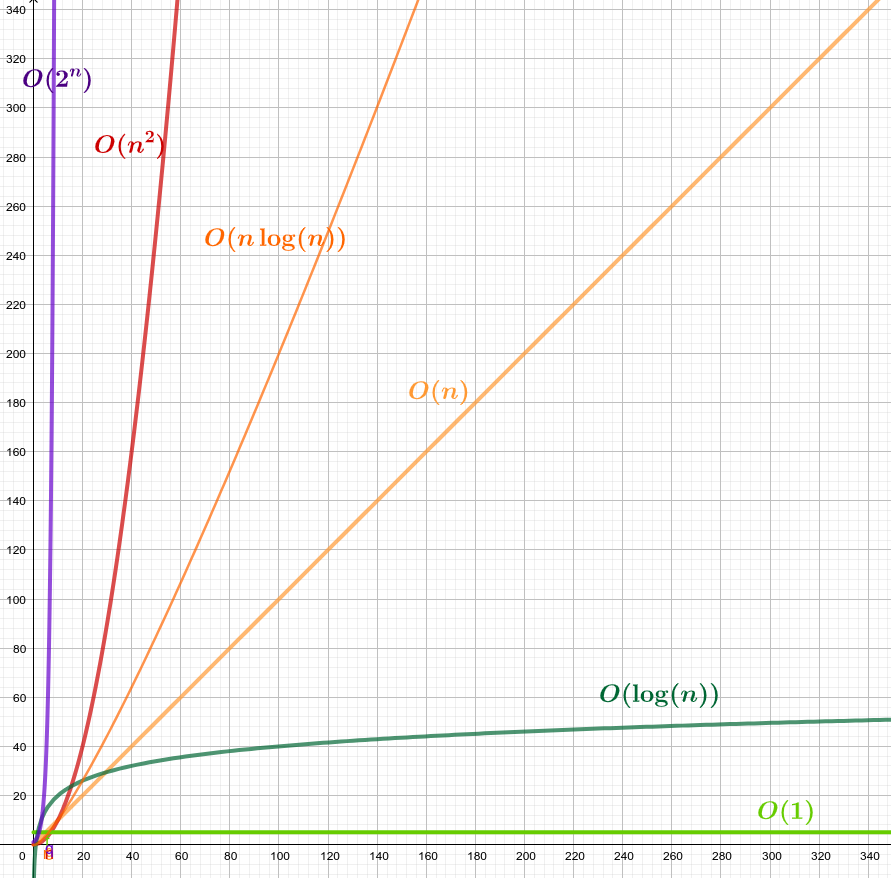
\includegraphics[height=6cm]{complexite.eps}
		\end{center}
	\end{block}
\end{frame}

\begin{frame}[fragile]{\Ctitle}{\stitle}
	\begin{block}{Temps de calcul effectif}
		Sur un ordinateur réalisant 100 million d'opérations par seconde :
		\renewcommand{\arraystretch}{1.3}
		\begin{tabular}{|c|c|c|c|c|c|}
			\hline
			\textcolor{blue}{Complexité} & $n=10$                      & $n=100$                     & $n=1000$                    & $n=10^6$                    & $n=10^9$                      \\
			\hline
			$O(\log(n))$   & \textcolor{green}{\faCheck} & \textcolor{green}{\faCheck} & \textcolor{green}{\faCheck} & \textcolor{green}{\faCheck} & \textcolor{green}{\faCheck} \\
			\hline
			$O(n)$   & \textcolor{green}{\faCheck} & \textcolor{green}{\faCheck} & \textcolor{green}{\faCheck} & \textcolor{green}{\faCheck} & $\simeq 10$s \\
			\hline
			$O(n)\log(n)$   & \textcolor{green}{\faCheck} & \textcolor{green}{\faCheck} & \textcolor{green}{\faCheck} & \textcolor{green}{\faCheck} & $\simeq 1,5$ mn \\
			\hline
			$O(n^2)$   & \textcolor{green}{\faCheck} & \textcolor{green}{\faCheck} & \textcolor{green}{\faCheck} & $\simeq 3$ h & $\simeq 300$ ans \\
			\hline
			$O(2^n)$   & \textcolor{green}{\faCheck} &  \textcolor{red}{\faTimes} &  \textcolor{red}{\faTimes} &  \textcolor{red}{\faTimes} &  \textcolor{red}{\faTimes} \\
			\hline
		\end{tabular}
	\end{block}
\end{frame}

\begin{frame}[fragile]{\Ctitle}{\stitle}
	\begin{exampleblock}{Exemples}
		\begin{itemize}
			\item<1-> On suppose qu'on dispose d'un algorithme de complexité linéaire travaillant sur une liste, il traite une liste de \numprint{1000} éléments en \numprint{0.015} secondes. Donner une estimation du temps de calcul pour une liste de \numprint{250000} éléments.\\
				\onslide<2-> {\textcolor{OliveGreen}{La taille des données a été multiplié par 250, la complexité étant lineaire le temps de calcul sera aussi approximativement multiplié par 250. \\}}
				\onslide<3->{\textcolor{OliveGreen}{$0.015 \times 250 = 3.75$, on peut donc prévoir un temps de calcul d'environ 3,75 secondes}}
			\item<4-> Même question pour un algorithme de complexité quadratique qui traite une liste de \numprint{1000} éléments en \numprint{0.07} secondes.\\
				\onslide<5-> {\textcolor{OliveGreen}{La taille des données a été multiplié par 250, la complexité étant quadratique le temps de calcul sera  approximativement multiplié par $250^2=62500$ \\}}
				\onslide<6->{\textcolor{OliveGreen}{$0.07 \times 62\,500 = 4375$, on peut donc prévoir un temps de calcul d'environ $4\,375$ secondes, c'est à dire près d'une heure et 15 minutes !}}
		\end{itemize}
	\end{exampleblock}
\end{frame}

\begin{frame}[fragile]{\Ctitle}{\stitle}
	\begin{exampleblock}{Exemple : exponentiation rapide}
		\begin{enumerate}
			\item<1->{\small Combien faut-il faire de multiplications pour calculer $a^{13}$ avec la fonction}
				\inputpartPython{\SPATH/puissance.py}{}{\footnotesize}{1}{6}
			\item<2-> {\small Combien en faut-il si on procède de la façon suivante :}
				\begin{itemize}
					\item<3-> Calculer $a^6$, l'élever au carré et le multiplier par $a$.
					\item<4-> Pour calculer $a^6$,calculer $a^3$ et l'élever au carré.
					\item<5-> Pour calculer $a^3$, élever $a$ au carré et multiplier par $a$.
				\end{itemize}
			\item<6-> {\small Généraliser la méthode précédente au cas d'un exposant quelconque et en déduire une relation de récurrence entre $a^n$ et $a^\frac{n}{2}$ si $n$ et pair et $a^\frac{n-1}{2}$ sinon.}
			\item<7-> {\small Proposer une implémentation récursive de ce nouvel algorithme.}
			\item<8-> {\small Déterminer la complexité de chacun des deux algorithmes, conclure.}
		\end{enumerate}
	\end{exampleblock}
\end{frame}

\begin{frame}[fragile]{\Ctitle}{\stitle}
	\begin{exampleblock}{Exemple : exponentiation rapide}
		\begin{enumerate}
			\item<1-> \textcolor{OliveGreen}{Il faut faire 13 multiplications, puisque $a^{13}$ est calculé avec :\\
					$a^{13} = 1 \textcolor{BrickRed}{\times} a \textcolor{BrickRed}{\times} a\textcolor{BrickRed}{\times} a\textcolor{BrickRed}{\times} a\textcolor{BrickRed}{\times} a\textcolor{BrickRed}{\times} a\textcolor{BrickRed}{\times} a\textcolor{BrickRed}{\times} a\textcolor{BrickRed}{\times} a\textcolor{BrickRed}{\times} a\textcolor{BrickRed}{\times} a\textcolor{BrickRed}{\times} a\textcolor{BrickRed}{\times} a$}
			\item<2-> \textcolor{OliveGreen}{Dans ce cas, il ne faut que 5 multiplications en effet, on calcul $a^{13}$ avec : \\
					$a^{13} = \left( \left(a^{\textcolor{BrickRed}{2}} \textcolor{BrickRed}{\times} a \right)^{\textcolor{BrickRed}{2}} \right)^{\textcolor{BrickRed}{2}} \textcolor{BrickRed}{\times} a$}
			\item<3-> \textcolor{OliveGreen}{$\left\{ \begin{array}{lll}
							a^n & = & \left(a^\frac{n}{2}\right)^2, \ \mathrm{si\ } n  \mathrm{\ est\ paire} \\
							a^n & = & \left(a^\frac{n-1}{2}\right)^2\times a, \ \mathrm{sinon\ }\end{array} \right. $}
		\end{enumerate}
	\end{exampleblock}
\end{frame}

\begin{frame}[fragile]{\Ctitle}{\stitle}
	\begin{exampleblock}{Exponentiation rapide}
		\begin{enumerate}
			\addtocounter{enumi}{3}
			\item<1-> \textcolor{OliveGreen}{Implémentation en Python:}
				\inputpartC{\SPATH/puissance.py}{}{\footnotesize}{8}{15}
			\item<2->\textcolor{OliveGreen}{Le premier algorithme a une complexité linéaire, celui-ci a une complexité logarithmique. En effet, l'exposant est divisé par 2 à chaque appel récursif}
		\end{enumerate}
	\end{exampleblock}
\end{frame}


\end{document}
